\documentclass{beamer}

% Theme choice
\usetheme{Madrid}

% Optional packages
\usepackage{graphicx} % For including images
\usepackage{amsmath}  % For math symbols and formulas
\usepackage{hyperref} % For hyperlinks
\usepackage{tikz}     % For charts

% Title, author, date, and institute (optional)
\title[Parallel Programming. Handshake lesson]{Parallel Programming course. Handshake lesson}
\author{Obolenskiy Arseniy, Nesterov Alexander}
\institute{Nizhny Novgorod State University}

\date{\today} % or \date{Month Day, Year}

% Redefine the footline to display both the short title and the university name
\setbeamertemplate{footline}{
  \leavevmode%
  \hbox{%
    \begin{beamercolorbox}[wd=.45\paperwidth,ht=2.5ex,dp=1ex,leftskip=1em,center]{author in head/foot}%
        \usebeamerfont{author in head/foot}\insertshortinstitute % Displays the university name
    \end{beamercolorbox}%
    \begin{beamercolorbox}[wd=.45\paperwidth,ht=2.5ex,dp=1ex,leftskip=1em,center]{author in head/foot}%
      \usebeamerfont{author in head/foot}\insertshorttitle % Displays the short title
    \end{beamercolorbox}%
    \begin{beamercolorbox}[wd=.1\paperwidth,ht=2.5ex,dp=1ex,rightskip=1em,center]{author in head/foot}%
      \usebeamerfont{author in head/foot}\insertframenumber{} / \inserttotalframenumber
    \end{beamercolorbox}}%
  \vskip0pt%
}

\begin{document}

% Title slide
\begin{frame}
    \titlepage
\end{frame}

\begin{frame}{Today}
    \tableofcontents
\end{frame}

\section{Introduction}
\begin{frame}{Introduction}
    Parallel Programming Course \\
    Contacts:
    \begin{itemize}
        \item Nesterov Alexander \\
            E-mail: nesterov.alexander@outlook.com
        \item Obolenskiy Arseniy \\
            E-mail: me@gooddoog.ru
    \end{itemize}
\end{frame}


\section{Structure of overall course}

\begin{frame}{Structure of overall course}
    \begin{center}
        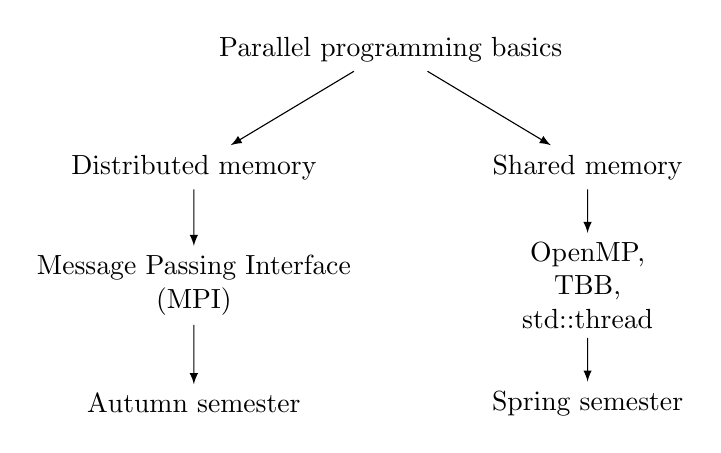
\begin{tikzpicture}
            [
                level 1/.style={sibling distance=50mm},
                level 2/.style={sibling distance=30mm},
                ->, >=latex
            ]
            \node {Parallel programming basics}
                child {
                    node {Distributed memory}
                    child {
                        node[align=center] {Message Passing Interface \\ (MPI)}
                        child {
                            node {Autumn semester}
                        }
                    }
                }
                child {
                    node {Shared memory}
                    child {
                        node[align=center] {OpenMP, \\ TBB, \\ std::thread}
                        child {
                            node {Spring semester}
                        }
                    }
                };
        \end{tikzpicture}
    \end{center}
\end{frame}

\section{Structure of the current semester}

\begin{frame}{Structure of the current semester}
    \begin{center}
        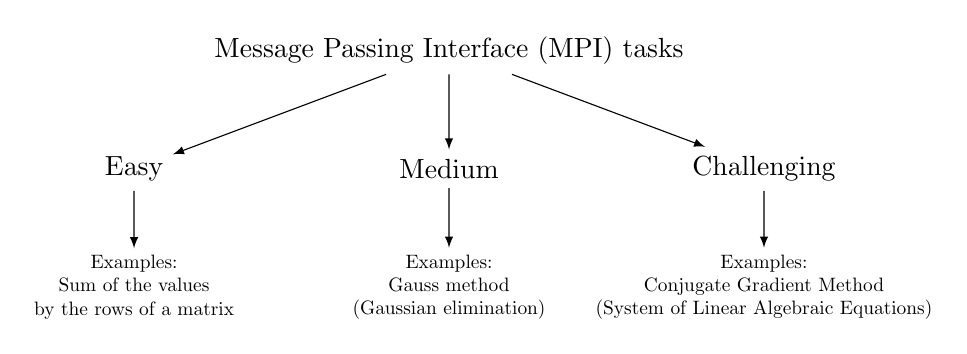
\begin{tikzpicture}
            [
                level 1/.style={sibling distance=40mm},
                level 2/.style={sibling distance=10mm},
                ->, >=latex
            ]
            \node {Message Passing Interface (MPI) tasks}
                child {
                    node {Easy}
                    child {
                        node[scale=0.7, align=center] {
                            Examples: \\
                            Sum of the values \\
                            by the rows of a matrix
                        }
                    }
                }
                child {
                    node {Medium}
                    child {
                        node[scale=0.7, align=center] {
                            Examples: \\
                            Gauss method \\
                            (Gaussian elimination)
                        }
                    }
                }
                child {
                    node {Challenging}
                    child {
                        node[scale=0.7, align=center] {
                            Examples: \\
                            Conjugate Gradient Method \\
                            (System of Linear Algebraic Equations)
                        }
                    }
                };
        \end{tikzpicture}
    \end{center}
\end{frame}

\section{Practice details}

\begin{frame}{Practice details}
    \begin{itemize}
        \item Practice format: Offline
        \item Random distribution of task variations
        \item Deadlines for each task
        \item Work organization in a single repository for all groups
        \item Self-review by students
        \item Full automation of quality and performance checks
        \item Optional reporting (written + spoken)
        \item Points-based grading system
        \item Plagiarism check of submitted tasks
        \item Main communication channel: Telegram
    \end{itemize}
\end{frame}

\begin{frame}{Points distribution}
    \begin{center}
        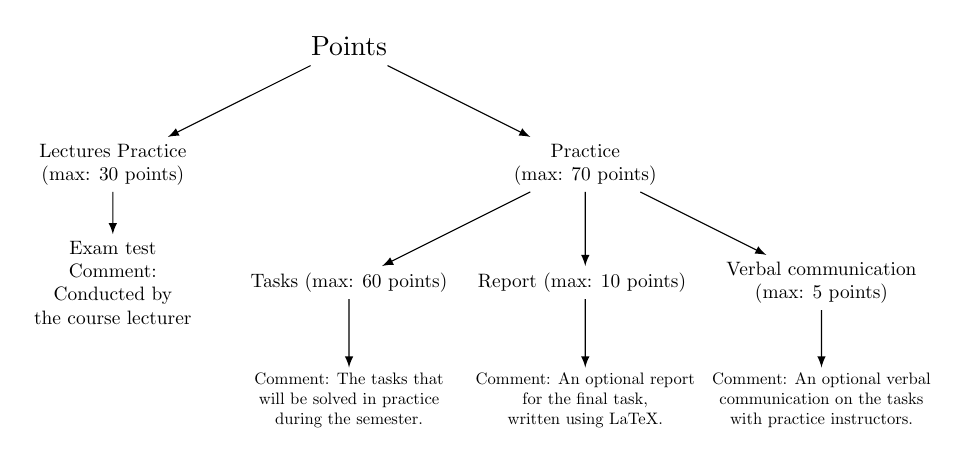
\begin{tikzpicture}
            [
                level 1/.style={sibling distance=60mm},
                level 2/.style={sibling distance=30mm},
                ->, >=latex
            ]
            \node {Points}
                child {
                    node[scale=0.7, align=center] {
                        Lectures
                        Practice \\
                        (max: 30 points)
                    }
                    child {
                        node[scale=0.7, align=center] {
                            Exam test \\
                            Comment: \\
                            Conducted by \\
                            the course lecturer
                        }
                    }
                }
                child {
                    node[scale=0.7, align=center] {
                        Practice \\
                        (max: 70 points)
                    }
                    child {
                        node [scale=0.7, align=center]{Tasks (max: 60 points)}
                        child {
                            node[scale=0.6, align=center] {
                                Comment: The tasks that \\
                                will be solved in practice \\
                                during the semester.
                            }
                        }
                    }
                    child {
                        node [scale=0.7, align=center]{
                            Report (max: 10 points)
                        }
                        child {
                            node[scale=0.6, align=center] {
                                Comment: An optional report \\
                                for the final task, \\
                                written using LaTeX.
                            }
                        }
                    }
                    child {
                        node [scale=0.7, align=center]{
                            Verbal communication \\
                            (max: 5 points)
                        }
                        child {
                            node[scale=0.6, align=center] {
                                Comment: An optional verbal \\
                                communication on the tasks \\
                                with practice instructors.
                            }
                        }
                    }
                };
        \end{tikzpicture}
    \end{center}
\end{frame}

\begin{frame}{Tasks points distribution (max: 60 points)}
    Easy tasks: 10
    \begin{itemize}
        \item Solution: 5
        \item Tests passed: 5
    \end{itemize}
    Medium tasks: 20
    \begin{itemize}
        \item Solution: 15
        \item Efficiency: 5
    \end{itemize}
    Challenging tasks: 30
    \begin{itemize}
        \item Solution: 20
        \item Efficiency: 10
    \end{itemize}
\end{frame}

\begin{frame}{Report and verbal communication (max: 15 points)}
    Report: 10
    \begin{itemize}
        \item The presence of the required items in the report format: 5
        \item Text quality and formatting: 5
    \end{itemize}
    Verbal communication: 5
    \begin{itemize}
        \item The completeness of the response: 5
    \end{itemize}
\end{frame}

\section{Administrative questions}

\begin{frame}{Assessments schedule}
    \begin{center}
        
\begin{tikzpicture}
            [
                level 1/.style={sibling distance=40mm},
                ->, >=latex
            ]
            \node {Assessments}
                child {
                    node [scale=0.7, align=center] {
                        Fundamental informatics \\
                        Autumn: Exam \\
                        Spring: Exam
                    }
                }
                child {
                    node [scale=0.7, align=center] {
                        Software enginerring \\
                        Autumn: Test (pass/fail) \\
                        Spring: Exam
                    }
                }
                child {
                    node [scale=0.7, align=center] {
                        Applied maths and informatics \\
                        Autumn: Test (pass/fail) \\
                        Spring: Test (pass/fail)
                    }
                };
        \end{tikzpicture}
    \end{center}
\end{frame}

\begin{frame}{Mark criterias}
    \begin{itemize}
        \item 5.5 (superb) - 99-100 points
        \item 5 (excellent) - 92-98 points
        \item 4.5 (very good) - 82-91 points
        \item 4 (good) - 70-81 points
        \item 3 (satisfactory or pass) - 50-69 points
        \item below - fail
    \end{itemize}
\end{frame}

\section{What will be covered in the next practice?}

\begin{frame}{Next steps}
    Practice 1 (intro)
    \begin{itemize}
        \item Tasks distribution
        \item A brief technical talk on parallelism
        \item Examples of MPI programs
    \end{itemize}
    Practice 2 (repo usage)
    \begin{itemize}
        \item Technical description of the repository and its checks
        \item Examples of project structure
    \end{itemize}
    Next practices (TBD)
\end{frame}

\section{Q\&A section}

\begin{frame}{Q\&A}
    \centering
    Any questions?
\end{frame}

\begin{frame}
    \centering
    \Huge{Thank You!}
\end{frame}

\end{document}
